%\documentclass[times]{MGS_class}
%%-----
%%Title und Author angeben
%\title{Software Maintenance in Game Engineering}
%\author{Michael Knett, BSc \textsuperscript{1} und David Portisch, BSc \textsuperscript{1}}
%%die Institute weiter unten zu den zugehörigen superscripts angeben
%
%\begin{document}
%
%\twocolumn[{\csname @twocolumnfalse\endcsname
%\begin{center}
%\maketitle
%%\thispagestyle{empty}
%
%%------
%%ANGABE DER INSTITUTE ANFANG
%
%\noindent \scriptsize \textsuperscript{1}\textsl{FH Technikum Wien, Game Engineering und Simulation, Wien, AUT}\\
%
%%ANGABE DER INSTITUTE ENDE
%%------
%\end{center}
%%\normalsize
%\hspace{15mm}
%
%}]%---

\begin{abstract}
Software Maintenance is an integral part of today's software life cycles, which also accounts for the development of video games. Even though maintenance has not historically received the same amount of attention like the other phases of the software life cycle, it forms a crucial part of software development as well. This paper is about the basics of Software Maintenance with a focus on how these are used in game development. In order to understand how maintenance is used in the development of video games, the general field of Software Maintenance is examined in this paper first. The term of Software Maintenance is elaborated and the different types of maintenance are discussed. Then the general maintenance process as well as some techniques for maintenance are described. The next part of this paper will focus on the most common forms of maintenance used in the gaming industry. This part will also show how the maintenance techniques in the gaming industry evolved over time. Finally, the topic of Community Feedback in video games is discussed. A case study of the handling of Community Feedback in the game Asterix \& Friends shows how Community Feedback can be managed in the development of a browsergame. 
\end{abstract}
\begin{keywords}
Software, Maintenance, Game Engineering, Patching, Updates, Community Feedback
\end{keywords}

\section{Definition}
\label{sec:definition}

Included in the life cycle paradigm for software, Software Maintenance forms an integral part of the software life cycle. Historically, the development part was categorized with more importance than maintenance. In general the other phases of the life cycle have received more attention than the maintenance part. However, this is now changing, as organizations try to keep the software operating as long as possible in order to gain the most out of their development investments.\citep{pigoski_software_2015}

The result of software development is typically a program which satisfies the user requirements. However, the software product also needs to adapt and evolve when in operation in response to changes. This can be due to environmental changes, new user requirements or anomalies which are uncovered during the operation of the software. The maintenance phase in the life cycle of the software starts with the delivery of the product, but the maintenance activities start much earlier.\citep{pigoski_software_2015}

Software Maintenance and maintenance in general are also formally described by ISO and IEEE Standards. The process of Software Maintenance is described in the IEEE 1219 Standard for Software Maintenance. It is described as the modification of a software product after its delivery in order to correct faults, improve its performance or adapt the software product in response to a changed environment. Maintenance activities prior to the delivery of the software product are also described in the standard, but only as an information annex. Furthermore, maintenance is described as one of the primary life cycle processes in the ISO/IEC 12207 Standard for Life Cycle Processes. The ISO/IEC 14764 International Standard for Software Maintenance describes the term similar to ISO/IEC 12207, but in this standard the focus is more on the aspects of maintenance before the delivery of the software product.\citep{pigoski_software_2015}

Studies and surveys show that the major part of maintenance, over 80\%, is used for non-corrective actions. This affirms that software evolves over its life cycle and thus maintenance is similar to software development, although it has its own unique processes. However, in contrast there is the common perception that maintenance is merely fixing bugs. This misconception originates from users who submit problem reports, which are in reality enhancement reports.\citep{pigoski_software_2015}

Software Maintenance is needed to ensure that the software product satisfies the user requirements over time. \textit{Pigoski} lists the following reasons why maintenance has to be performed:\citep{pigoski_software_2015}

\begin{itemize}
    \item Correcting errors
    \item Correcting requirements and design flaws
    \item Improving the design
    \item Making enhancements
    \item Interfacing with other systems
    \item Converting programs so that different hardware, software, system features, and telecommunications facilities can be used.
    \item Migrating legacy systems
    \item Retiring systems
\end{itemize}

Even though Software Maintenance activities are similar to those of software development, there are unique activities bound to Software Maintenance as well. Analysis, design, coding, testing and documentation are done by maintainers as well. Requirements are tracked and worked on just as in traditional software development. \textit{Pigoski} mentions in \citep{pigoski_software_2015} the following Software Maintenance activities: \citep{pigoski_software_2015} 

\begin{itemize}
    \item \textbf{Unique Activities}\newline
    Problem solving skills are very important for software maintainers. They have to analyze change requests, translate these into software terms and then identify the affected components. This gets even more complicated, if the maintainer has to maintain a software written by a third party. Furthermore, the maintainer needs intimate knowledge of the softwares code and its structure. This is used to perform an impact analysis, which identifies all the systems and system products affected by a change request. Finally the risk of actually implementig the change is determined, several potential solutions are provided and a recommendation for the best possible course of action is made.\citep{pigoski_software_2015} 
    
    \item \textbf{Supporting Activities} \newline
    Supporting Activities like Configuration Management or Quality Assurance can also be performed by a maintainer.\citep{pigoski_software_2015}
    
    In IEEE 1219, the IEEE Standard for Software Maintenance, Configuration Management is listed as a critical part of the maintenance process. The modification request and problem reports need not only to be tracked. This is not sufficient. It is also important to control the software product and any changes made to it. This can be done by enforcing a Software Configuration Management process. \citep{pigoski_software_2015}
    
    Concerning quality it is more than just hoping that maintenance will increase the quality of the product. This needs to be planned and processes must be set up in order to support the maintenance of the software. \citep{pigoski_software_2015}
    
    Another important point is the Maintenance Planning Activity. The maintenance phase typically lasts for several years and thus accurate planning of resource needs is a key factor in maintenance planning. It is very important to include these resources, which include cost, into the project planning budget. Thus Maintenance Planning and the development of a maintenance plan should begin with the start of the project. This maintenance plan should be prepared during the development of the software product and address how the users will request modifications or report problems. \citep{pigoski_software_2015}
\end{itemize}

\subsection{Role of a Maintenance Programmer}
\label{subsec:roleMaintenanceProgrammer}

As indicated before, problem solving skills are crucial for maintenance programmers as they need to analyze change requests, then translate them into software terms and finally identify the affected components. The maintenance programmer also needs to keep track of the changes made to the software through a Configuration Management Process.\citep{pigoski_software_2015}

A challenge faced by a Maintenance Programmer can be a limited understanding of the maintained software. 40\% to 60\% of the time, as indicated by practitioners and researchers, is used for understanding the software to be modified/maintained. So program comprehension should be one of the key interests of a Maintenance Programmer. Often maintainers have a limited understanding of the software they maintain and therefore need to acquire the knowledge about the software on their own, which can be even more difficult, if the software is not documented well.\citep{pigoski_software_2015}

\section{Types of maintenance}
\label{sec:typesOfMaintenance}
Maintenance is commonly divided into three parts. \citep{cote_model_1990} \newline
Perfective maintenance, which is about improving the product, takes up about 60\% of the total time spent on maintenance. Corrective maintenance takes up about 18\% and is about fixing bugs. Adaptive maintenance corresponds to adapting the application to a changed environment and takes up 18\%. The remaining 4\% are used on other forms of maintenance.\citep{jarman_testing_2010}

These three different categories of maintenance (corrective, adaptive and perfective maintenance) were originally created by E.B. Swanson of UCLA. By using empirical data from the industry Swanson was one of the first to be able to examine what really happens in software evolution and maintenance.\citep{pigoski_software_2015}

\subsection{Perfective Maintenance}
\label{subsec:perfectiveMaintenance}
Perfective maintenance is defined by the Institute of Electrical and Electronic Engineers(IEEE) as "Modification of a software product after delivery to improve performance or maintainability". \citep{ieee_software_1998} This definition is very important for the game industry. Due to this every performance improvement, added feature or downloadable content(DLC) is considered to be perfective maintenance.

Thus the two goals of perfective maintenance are to improve \textit{performance} and \textit{other attributes} of the product. Both goals are achieved by applying tuning measures. Improving \textit{performance}, also called \textit{optimizing}, describes for example reducing the response time of the application or reducing the memory usage. The \textit{improvement of other attributes} of the product is also called \textit{Re-engineering}. In this context Re-engineering describes a technical improvement of the system. It shall be easier to operate, maintain and extend the software.\citep{sneed_software_2005}

The most widely used way for perfective maintenance in the game industry is for the use of DLC.\citep{jarman_testing_2010} The strategy of developers is to release some downloadable content a few months after the release of their game.\citep{jarman_testing_2010} This DLC can either be free or paid. The reason behind this is to extend the attention a game has for a few months more in order to get additional customers and keep existing ones happy.\citep{jarman_testing_2010} With the use of this strategy developers can get an added income to keep maintaining the game after its release or divert the funds towards their next game.\citep{jarman_testing_2010} Maintenance developers also get an additional feedback loop for their work. \citep{jarman_testing_2010}

The Internet has revolutionized the perfective maintenance in the game industry, due to its easy ability to transmit patches and downloadable content. \citep{jarman_testing_2010} Before this, when a bug or glitch was discovered, the only way to patch a game was to release an expansion, which in turn could introduce even more bugs. \citep{jarman_testing_2010}

However, when optimizing or re-engineering the software, it implies that this is a planned change of the system in order to improve it. Thus it needs to be defined, what is actually an improvement of the system, how high the effort to achieve this is and whether this is cost-effective.\citep{sneed_software_2005}


\subsection{Corrective Maintenance}
\label{subsec:correctiveMaintenance}
Corrective maintenance is used after an applications initial release. It is the process to find and fix any bugs that have made it through testing.\citep{jarman_testing_2010} Thus corrective maintenance is a reactive modification of the software product after its delivery.\citep{pigoski_software_2015} The corrective maintenance then produces a patch which can be distributed via a network. These can be manually distributed or applied automatically via a download service like Steam or PSN. \citep{jarman_testing_2010} 

Corrective maintenance may also be needed after a perfective maintenance, because adding code and features increases the chances for more programming errors. \citep{jarman_testing_2010} \newline
For example, game developers may find players actively seeking and exploiting features in their game. Therefore glitching or breaking the game by accessing areas that were never meant to be explored or simply using a feature in a clever way and making it unbalanced.\citep{moore_game_2009}

Developers can fix issues as they arise, but by doing so, this can lead to more problems. To be able to correct code one needs to change code which, by it's nature, can lead to even more bugs. This type of error is named regression fault. In order to fix these issues even more corrective maintenance needs to be done, until all bugs have been erased. \citep{moore_game_2009}

The defects which are addressed by corrective maintenance range from minor to serious major defects. The level of the defect depends on how much the defect affects the usability of the program and its environment. E.g. if a memory access error overwrites some data and the program continues running, the following results of the program are corrupted. The system is not usable anymore in this state and thus this is a serious defect. In contrast, it may be irritating if some text in the user interface is not correctly written, but this does not prevent using the program in most cases. Therefore this defect falls into the category of minor defects. The circumstances and the financial consequences of these two defects are entirely different and thus a major defect can weight 100 to 1000 times more than a minor defect.\citep{sneed_software_2005}

\begin{strip}
    \centering\noindent
    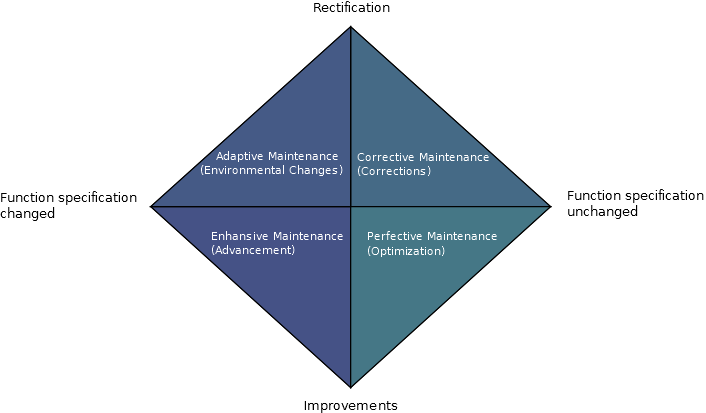
\includegraphics[width=\linewidth]{img/MaintenanceTypes.png}
    \captionof{figure}{\protect This figure which was adapted from the figure \textit{Abb. 1-5} from  \citep{pigoski_software_2015} shows the four main activities of Software Maintenance and enhancement. Adaptive maintenance, corrective maintenance and perfective maintenance belong to the field of Software Maintenance. In contrast enhansive maintenance belongs to the field of Software enhancement, because it represents an addition to the products' features through enhancing the software. Thus it is different to adaptive maintenance where the products' features are not increased, but rather adapted to a changed environment.\citep{pigoski_software_2015}}
\end{strip}

\ 
\pagebreak
\ 
\linebreak
\pagebreak % This hack is even uglier, but at least it looks funny :)

Therefore the corrective maintenance is divided into these categories \citep{sneed_software_2005}:
\begin{itemize}
    \item \textbf{Maintenance and repair} This category deals with repair of the major defects. It is event driven and needs to react as soon as a major defect occurs. Thus an emergency service needs to be setup.
    
    \item \textbf{Defect Correction} Correcting minor defects is addressed by this category. The correction of these defects can be planned, because they do not prevent the operation of the software. Normally they are corrected all at once with the new release of the product.
\end{itemize}



\subsection{Adaptive Maintenance}
\label{subsec:adaptiveMaintenance}
When an environment, where a game is running, is changed adaptive maintenance is used.\citep{jarman_testing_2010} The software is modified after its delivery in order to keep it still usable in a changed or changing environment.\citep{pigoski_software_2015} For example, if a new firmware update for a console is being released and a developer needs to change some code, otherwise it wouldn't work, this is called adaptive maintenance. Games are usually not effected by changes to the environment, especially on consoles.\citep{jarman_testing_2010}

For software systems there are two types of environments which can change: First there is the functional environment where for example laws, specifications or business rules can change. On the other side there is the technical environment where for example Database-Systems, Operating Systems, the hardware or as mentioned before the firmware can change. Adaption is considered as the most important type of maintenance, because without advancement the software will \textit{die}.\citep{sneed_software_2005}

\subsection{Preventive Maintenance}
\label{subsec:preventiveMaintenance}
Preventive maintenance, which was introduced after perfective, corrective and adaptive maintenance, is performed in order to prevent problems from happening. It is defined as a modification of the software after its delivery in order to detect and correct hidden faults, before they actually become active faults. Thus this type of maintenance is most often used in software systems where safety is a crucial concern.\citep{pigoski_software_2015}

%\begin{figure}[!htbp]
%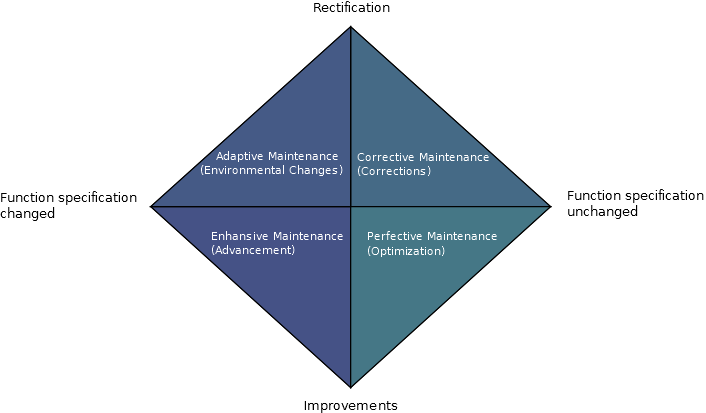
\includegraphics[width=1.0\columnwidth]{img/MaintenanceTypes.png}
%\caption{ caption \protect with citation \citep{pigoski_software_2015}}
%\label{fig:maintenanceTypes}
%\end{figure}

\section{Techniques for Maintenance}
\label{subsec:techniques}

Techniques specific to maintenance can be used in order to achieve effective Software Maintenance. \textit{Pigoski} lists in \citep{pigoski_software_2015} the following maintenance techniques: \citep{pigoski_software_2015}

\begin{itemize}
    \item \textbf{Program Comprehension}\newline
    Programmers spend a considerable amount of time in reading and comprehending source code in order to implement changes. Thus it is crucial to aid this process with tools, techniques and processes. A key tool for the program comprehension are code browsers and an understandable and concise documentation can aid greatly as well. \citep{pigoski_software_2015}
    
    \item \textbf{Re-engineering}\newline
    In re-engineering a system is first examined and then changed in order to recreate it in a new form. This also includes the subsequent implementation of the new form of the system. Often re-engineering is not used in order to increase maintainability, but rather to replace aging legacy systems. \citep{pigoski_software_2015}
    
    \item \textbf{Reverse engineering}\newline
    Reverse engineering is the process of analyzing a subject system in order to get a higher level abstraction of it which is easier to comprehend. Thereby the system's components and their interconnection are identified to create this high level representation of the system. Reverse engineering is a passive process, because it does not change the system in any way nor does it yield a new system. There are different types of reverse engineering like re-documentation, design recovery and data reverse engineering. \citep{pigoski_software_2015}
    
    \item \textbf{Impact Analysis}\newline
    Impact analysis has two major tasks. First it checks which systems and system products are affected by a change request and second it estimates the resources which are needed in order to implement this change. This process is performed after a change request enters the configuration management. \citep{pigoski_software_2015}
\end{itemize}

\section{Maintenance in Game Engineering}
\label{sec:maintenanceGameEngineering}
This chapter shall give an overview over terminology and techniques concerning maintenance in the area of Game Engineering.

\subsection{Maintenance Terminology in Game Development}
\label{subsec:typeGameEngineering}
\begin{itemize}
    \item \textbf{Hotfix}\newline
    When a critical bug is found in the live-environment it needs to be fixed as soon as possible. If this can be done, without taking down the  live-environment, then this is called a Hotfix. For example in a server-client environment this could only affect the server-side. That means the user would not need to restart and update their client. A Hotfix is generally made outside of normal testing-procedures, which means it is more error prone and does not guarantee that it will fix the problem. This is corrective maintenance.\citep{seibert_interview_2016}
    \item \textbf{Bugfix}\newline
    When a critical bug is found, and the environment needs to be taken down in order to fix it, then this is called a Bugfix. A Bugfix should be tested beforehand to confirm that it really fixed the issue. Bugfixes are usually grouped together before they are deployed, so the user only needs to update their client once. This is corrective maintenance.\citep{seibert_interview_2016}
    \item \textbf{Tweak}\newline
    A deployed/existing feature needs to be adjusted. This can be a combination of several hotfixes on the server and bugfixes on the client side. Depending on the situation, this can be adaptive or corrective maintenance.\citep{seibert_interview_2016}
    \item \textbf{Content/Feature - Update}\newline
    New Content and Features are a type of perfective maintenance.
    \item \textbf{Technical Maintenance}\newline
    When the server-infrastructure needs to be updated, or another server needs to be added, that is called technical maintenance. Theses things are usually met with a small downtime of the system and is done at a time where the least amount of users are active. This is adaptive maintenance.\citep{seibert_interview_2016}
\end{itemize}

\subsection{Maintenance techniques in the early game industry}
\label{subsec:techniquesEarlyGameIndustry}
In the early game industry global Internet access for the general public was a far of dream. So games that were developed needed to be as bug-free as possible because released games had only a very limited amount of methods available to deploy patches.\citep{jarman_testing_2010}
\begin{itemize}
    \item \textbf{Addon/Sequel}\newline
    One way to deliver a patch to the user is via addons. Addons are expansions of the original game content. Additional content however, can introduce new bugs as well.\citep{jarman_testing_2010}
    \item \textbf{Re-Release}\newline
    Another form of delivering a patched version to the user is with a re-release of the game. This was also one of the earliest form of DLC as developers could attach new content to the re-released version as well. For the user however, this meant they had to buy the same game again if they wanted a patched version or the new content. \citep{jarman_testing_2010}
    \item \textbf{Manual Patching}\newline
    With the rise of the Internet game developers were creating patches for their games more frequently. They then made them available on their (or other) websites for users to download and apply manually. Care needs to be taken when installing such patches as the version prior to the installation needs to match the patch as well.\citep{jarman_testing_2010}
\end{itemize}

\subsection{Today's maintenance techniques in the game industry}
\label{subsec:techniquesTodaysGameIndustry}
In modern times most users have access to the Internet. Therefore delivering a patch to the user is easier than before.
This however can lead developers to code sloppier because they can just patch it afterwards\citep{jarman_testing_2010}. Companies will try to release their games when no other major game is being released, as to not split the customer attention to multiple games and therefore potentially splitting profits for both games \citep{jarman_testing_2010}. When a critical bug is found, that for example prevents the game to be finished under certain circumstances, then usually a game is delayed. On the other hand, the game could be released and later be patched as soon as possible. This would give the image that the company is lazy and unprofessional, which can lessen the profit made\citep{jarman_testing_2010}.

An obvious advancement of the earlier manual patching is an automated patching process. This can either be done via a download platform, like Steam or PSN, or via the games own launcher.

It is inevitable that software, especially games, have a need for change. These changes happen mostly because of a changing environment.\citep{bcs_software_2015} \newline
One possible approach is to design, develop and maintain a system that is easy to change and each change should have as few impact as possible on the whole system. \citep{bcs_software_2015} This is known as Change Isolation. Methods that can utilize this can range from code level construction of classes, memory management or even up to a business level purchase of new servers and how to change or integrate them into an existing server cluster.\citep{bcs_software_2015} \newline
Change Isolation can give us:
\begin{itemize}
    \item Break a complex implementation into a modular design that can be easier understood and maintained.
    \item Extend a system/modules lifespan.
    \item Breaking down code results in modules/components that can be reused.
\end{itemize}

For example in \textit{Bungie}'s old \textit{blam} engine, which was used for e.g. the \textit{Halo} games, the game code was accessible from any layer of the engine. This may sound great, because it simplifies the development of the game a bit, but the true implication was that it was hard to share code between their games. The reason for this was that the engine was tainted with game logic, which of course was not used in the next games. This is a point which the development team at \textit{Bungie} took into account, when they developed their new engine for the game \textit{Destiny}.\citep{butcher_destiny_2015}

However, \textit{Change Isolation} is not always fully applicable. \textit{Butcher} from the company \textit{Bungie} explains in his talk \citep{butcher_destiny_2015} about the development of their new engine for the game \textit{Destiny} that the dependencies of modules in different levels of the engines are stronger or weaker according to the layer they are in. He differentiates between the \textit{Core-Engine} and the \textit{Feature Components}. The \textit{Core-Engine} are features which other engine features are built upon like Application Lifecycle, Resource Management, Streaming System, Core Render Architecture or the Core Content Pipeline. \textit{Butcher} mentions that these \textit{Core-Engine} features tend to be tightly coupled into on another because they have shared assumptions about data formats, object lifetime, state management and multithreading. Every component needs to follow these \textit{rules} or else the game is buggy and/or unstable. This is one of the reasons why the development team decided to develop a new engine. The old \textit{blam} engine had shared assumptions like single-threading, one platform, and a simple content pipeline which had no system for patching content post-release. The \textit{Feature Components} in contrast build up upon the Core-Engine and tend to be more loosely coupled and talk to each other through interfaces.\citep{butcher_destiny_2015}

\section{Software Maintenance Guide}
\label{sec:softwareMaintenanceGuide}

Event though the maintenance phase of a software starts with the delivery of the product, the maintenance activities start much earlier.\citep{pigoski_software_2015} This section shall give an overview over how maintenance can be integrated into the development of software.

The development of a software can be categorized into the five different phases of product life-cycle. At each stage a different amount of maintenance happens:

\begin{itemize}
    \item \textbf{Planning Phase}

    Even in the planning phase maintenance should be considered. Creating coding guidelines can be used to structure code in a unified way, making maintenance work easier later on. The scalability of the software/game should be taking into consideration as well. Adaptive maintenance is, for example, used when upgrading a server infrastructure to take a heavier load during peak hours. It can therefore be planned that the servers can be swapped out for a newer generation or simply upgraded in their number. Of course the software needs to be prepared for this scenario.

    \item \textbf{Development Phase}

    During the development phase of a software product the software is usually developed in the three sub phases of \textit{Design}, \textit{Programming} and \textit{Testing}. These phases are repeated over and over and can lead to a change in the technical concept of the product. Thus correction, adaption and extension of the technical concept is performed during the development phase and can be seen as the first work on System Maintenance.\citep{pigoski_software_2015}

    \item \textbf{Evolution Phase}

    The first big Software Maintenance occurs during the \textit{Evolution Phase}. The Software Product is still extended, but the main focus lies on the maintenance of the software version which is used in production. This is a critical task and has the highest priority. Corrective maintenance and adaptive maintenance is now used to correct the occurring defects and perform adaptions. The least priority has the task of enhancement of the software product. In the Evolution Phase re-engineering can be performed as well, to achieve technical perfection. However, most times there is not much time left from the three previously described fields, so that in practice re-engineering is only performed in emergencies.\citep{pigoski_software_2015}

    \item \textbf{Maintenance Phase}

    During the Maintenance Phase only maintenance and correction are performed with a limited capacity. This phase starts, when the software product can't be enhanced anymore and thus only needs to be kept running anymore.\citep{pigoski_software_2015}

    \item \textbf{Retirement Phase}

    If for example the functionality of the software does not suit its usage, it is retired. It may be that the system is still used by some users and thus it can still stay in production for a while. However, in this phase no maintenance happens anymore.\citep{sneed_software_2005}
\end{itemize}

Besides the software life-cycle according to \citep{sneed_software_2005} the software maintenance activity in the development can be divided into three parts\citep{sneed_software_2005}:
\begin{itemize}
    \item \textbf{Maintenance and repair service} For the immediate correction of major defects.
    
    \item \textbf{Rectification service} For the periodic adaption of the system to a changed environment and the correction of minor defects.
    
    \item \textbf{Re-engineering service} Responsible for the occasional revision of the system (perfective maintenance)
\end{itemize}

As soon as the maintenance activities for a project are set up, these three parts can be found in all the phases of the software development life-cycle.

When maintaining the project the \textit{process of change} needs to be taken into account. As iterations of changes happen, mostly through adaptive or perfective maintenance, the system will slowly drift apart from the original design. The system may still give the originally intended output, but it can use different algorithms than it's creators intended. This is called \textsl{structural decay}.\citep{bcs_software_2015} \newline
Structural decay needs to be kept in check with a design that is focused on change and documentation.\citep{bcs_software_2015} Otherwise a system slowly becomes unmaintainable because future maintenance developers will have no idea how much of the original documentation is still valid. Examples can be found in big companies where undocumented legacy systems are still used because of the fear that some small change could break everything.

\section{Community Feedback}
\label{sec:communityFeedback}

\subsection{Maintenance and Community Feedback}
\label{subsec:maintenanceAndCommunityFeedback}
Some types of maintenance have to do with improving the product (perfective maintenance) or fixing bugs (corrective maintenance). In the development of games Community Feedback can be used as a tool to support these maintenance types, but also to be a part of the whole development process. This accounts for MMOs, browsergames, but also for games which are in \textit{early access} and/or funded via crowd funding.

In his talk \citep{lierop_community_2015} at GDC about \textit{The Long Dark \& Community Influenced Development} Lierop depicts the way of \textit{Community informed Development}. He describes it as \textquotedblleft A process by which you take feedback from your community and incorporate it into your decision-making"\citep{lierop_community_2015}. It is important that this does not mean that they make the game the community wants. They are developing the game they want to make with the community as a sounding board of ideas.\citep{lierop_community_2015} This is quite similar to the approach \textit{Sproing Interactive Media GmbH} is following with the development of the Browser Game \textit{Asterix \& Friends} concerning Community Feedback. They gather feedback from the community, listen to them, but finally the development team themselves decides what is implemented and what not.\citep{seibert_interview_2016}

So there is a huge difference between \textit{asking the community to give you feedback} and \textit{asking the community to tell you what to make}. Asking the community for feedback involves them into the process of refinement (like \textit{perfective maintenance}) and the developers have the chance to test out ideas. On the other hand, asking the community to tell the developers what to make puts the players into the \textit{driver's seat}. However, the gamers are not equipped to do this.\citep{lierop_community_2015} Some gamers may also have a very strong interest into video games as a medium and have informed themselves about the development process, but they don't have the same knowledge about the game as a game designer of the game has. Thus they may have a great idea, but are not aware of the implications the idea has on the game as a whole, which a game designer of the development team is aware of in contrast.\citep{seibert_interview_2016} If the developers listen to the opinions and suggestions of the players all the time, it is very likely that the finished game does not represent the team's strong vision of the game as it would have otherwise. The community can rather be seen as another voice which the developers can listen to in order to improve the game.\citep{lierop_community_2015}

This way of game development is quite different from the traditional way. With this way of development early on from the beginning of the development of the game, the developers can test out ideas in the concept development phase. This means that feedback is gathered early on from the community and the developers try to understand what they like. It is a \textit{live} development similar to the development of an MMO and browser-games. There is a direct connection to the community and feedback is flowing in both directions. Thus this is a much more transparent process. The developers have direct access to the community and vice versa.\citep{lierop_community_2015}

In comparison the traditional way of game development is mostly performed in secret, until the project is done and released. There is very little input from outside and thus also very little validation. Often the result is then misaligned with the expectations of the audience. Furthermore, the communication is mostly done by the PR and marketing.\citep{lierop_community_2015}

Besides all the Community Feedback it is important to perform analytics as well. This is essential, because the people who comment and give feedback the most do not need to be the majority of the people who play the game. A good example of this happened during the development of the game \textit{The Long Dark}. With the feedback from the community the developers of \textit{The Long Dark} could identify two types of players who play their game. On the one hand they had players who wanted an emotional experience in the game and enjoy the atmosphere. But on the other hand there were players who wanted a hardcore survival experience with the game. So the team introduced three different experience modes in the game which differ for example in difficulty: First there is the \textit{Pilgrim} mode, which is for the players who want an emotional experience from the game and enjoy the atmosphere. The \textit{Hardcore} mode offers a hardcore simulation and the \textit{Voyageur} mode lies in the middle of the other two experience modes. Interestingly, the hardcore gamers tended to be more engaged with the game, commented a lot more and gave a much feedback. If the developers had only read the comments and feedback about their game, they may would have come to the conclusion that the majority of their player-base are hardcore players. However, according to the metrics the developers collected with the analytics, about 60\% of their players played the \textit{Voyageur} mode, about 25\% the \textit{Pilgrim} and only about 12\% picked the \textit{Hardcore} mode. So in reality the majority of the comments and feedback did not represent the majority of the player base. Thus it is important to perform analytics and collect metrics as well in order get objective data. The developers should understand how the players of their game actually break down in categories, or they could think that the players who give the most comments or feedback form the whole of their community, which does not have to be true.\citep{lierop_community_2015}

According to \textit{Lierop} in \citep{lierop_community_2015} it is important that the developers stay to their vision. Community feedback can be a valuable tool, but it is also important to consider that this also implies risks to the direction and the vision of the game.\citep{lierop_community_2015}

\subsection{Community Feedback in Asterix \& Friends}
\label{subsec:communityFeedbackInAsterixAndFriends}
This chapter is a Case Study about the role of Community Feedback in the development of Asterix \& Friends. It is based on an interview via e-mail with Felix Seibert from Sproing Interactive Media GmbH which took place from 2015-12-16 to 2016-01-07.

Asterix \& Friends is a Free-2-Play browsergame based on the brand of \textit{Asterix and Obelix}. The player has to build up a gaul village and defend it against the Roman legionaries. Thereby the player needs to gather resources, refine them and construct buildings. Various tasks and missions need to be accomplished as well.\citep{asterix_faq_2014} The game is developed by Sproing Interactive Media GmbH and published by Sproing Publishing GmbH. It was released in April 2013 for PC.\citep{asterix_sproing_2015}

How Community Feedback is given depends a lot on how much a player knows about the development process of a video game in general. It is important that the game developer knows about that and it can help to be aware how much the players who give the Community Feedback know about the development process. In general there can be two types of players who give feedback:\citep{seibert_interview_2016}

\begin{itemize}
    \item Some players have a solid knowledge about the reality of game development. With a distinctive interest into the media of video games, they may inform themselves a lot about the development process of them as well. This has an impact on the feedback they give.
    
    \item For the other players this kind of knowledge is missing. They may like to play video games a lot, but don't deal with the development process of a game. Of course this has an influence on the feedback they give and can lead to utopistic requests which are not possible for the development team to implement.
\end{itemize}

Of course both types of players can give good suggestions, but it can help to keep in mind which types of these players mainly give feedback for the game.\citep{seibert_interview_2016}

In general Community Feedback for Asterix \& Friends is gathered via these four platforms:\citep{seibert_interview_2016}

\begin{itemize}
    \item \textbf{A forum}
    
    The \textit{forum} for the game also provides the possibility for the players to provide feedback.
    
     \item \textbf{A Support-form}
     
     Even though the primary purpose of the \textit{support form} is to report bugs, it can also be used to provide feedback about the game.
     
     \item \textbf{A Support-Address}
     
     The \textit{support address} works like the \textit{support form}, but it does not have the predetermined structure like the \textit{support form}.
     
     \item \textbf{Facebook}
     
     Feedback can be provided through the comment function of \textit{Facebook}.
\end{itemize}

With Community Feedback there is no guarantee of qualitative and elaborate feedback. Mostly the spontaneous feedback by the players, which was not explicitly asked for by the developers, can be a bit chaotic. For example Facebook comments are informally written and often only contain rough ideas than elaborated suggestions. In the forum \textit{idea threads} are also started where the players discuss their ideas on how the game could be improved or changed. The feedback through the support forms is a bit different. Most times these are more elaborate.\citep{seibert_interview_2016}

The development team of Asterix \& Friends has made better experiences, when they guided the process of the Community Feedback. This way they get feedback about topic which are relevant for the team at the moment. After an update a \textit{Feedback-Thread} is created in the forum or a link to a survey is posted on Facebook. However, spontaneous feedback is still very important for the team, because it can contain ideas and approaches which the development team didn't think of before.\citep{seibert_interview_2016}

In the development of \textit{Asterix \& Friends} all the essential design decisions are made by the development team. Concerning the Community Feedback this means that the team acts as a \textit{gatekeeper} who decides which changes or features are implemented and which are not. Thus the Community Feedback which is received by the development team is read and reviewed. Most times a member of the development team can evaluate right away, whether a suggestion can be implemented or not, because they know the restraints and constraints of their project. The development team of \textit{Asterix \& Friends} uses 4 aspects to review a suggestion from Community Feedback:\citep{seibert_interview_2016}

\begin{itemize}
    \item \textbf{Technical Constraints}
    
    Sometimes the technology which is used to build the game prevents a feature or a suggestion, because it is simply not possible to be implemented with it. In \textit{Asterix \& Friends} for example they got the suggestions from multiple players to change the chat, but that was not possible with the used technology. Changing the technology would be possible, but it would cost much time and effort and thus slow down the development of other features.
    
    \item \textbf{Good design}
    
    The more people are involved into the design process of game, the more difficult it is to maintain a clear vision of the game. Even though an idea is technically possible and well-thought-out, it may has implications on the game which are not good for the game as a whole. Thus the ideas also need to be checked by a designer who knows the game very well. \textit{Design by the fans} does not have to be a good thing, because even though a person likes to play the game very much, this does not mean that they know what is best for the game.
    
    \item \textbf{Resources}
    
    Every project in a company has to work with a contingent of resources they get assigned. Thus it is not possible to implement some suggestions, because there are not enough resources to do so. The implementation of some suggestions would require to increase the team size of the development team significantly which is very often no option.
    
    \item \textbf{Publisher and Licence holder}
    
    Ideas and suggestions can also be rejected by partners like publishers. \textit{Asterix \& Friends} is the game for a worldwide well-known brand and thus the development team has to follow strict licence specifications. Quite often this is the reason, why ideas had to be discarded. Even if lots of players wish a feature to be implemented, it may is impossible due to licence constraints.
\end{itemize}

According to these points the development team of \textit{Asterix \& Friends} decides whether a suggestion can be implemented or not. However, even if an idea is categorized as implementable, this does not mean that this will happen immediately. The idea or suggestion needs to be assigned to a developer and may also needs to be elaborated further. If this task then has a low priority it can take some time until it is finally developed and implemented. When the task is finally done it is tested on the development server and afterwards included in the next update for the live server.\citep{seibert_interview_2016}

The changes to the game are then documented, so that it is possible to retrace who, where and when changed what. This is essentially important if new people join the development team or existing members leave the team. For \textit{Asterix \& Friends} an internal wiki is used in the company to document the changes. All the changes on the live server are also documented in the patch notes which are also distributed to the players. However, for the patch notes it can be possible, that some changes are not included, because they are not relevant and visible for the players or the development team does not want share this piece of Information. Most times, the patch notes are published at the day of the update, or shortly before. This way the players know for sure what changed in the game and thus can give adequate feedback.\citep{seibert_interview_2016}

When a new feature or change is implemented the live server needs to be updated. For \textit{Asterix \& Friends} it was clear from the beginning of the development that there will be down times for the updates and the maintenance of the game and server. The development team follows the principle that there are down times when they are needed. Thus the server is updated, whenever there are enough new features and changes for an update, or if it is absolutely needed due to unavoidable technical changes and/or bugfixes. Down times are announced through all the communication channels in advance for the players. A good communication is needed so that the players are aware of the downtime. Furthermore, 30 minutes before the down time a timer is started in the game to make the players which are still in the game aware that the game won't be playable for a short time. The team tries to keep these down times as short as possible and tries to perform them when only a few players are online. Most times the down times for \textit{Asterix \& Friends} are performed in the late morning and the team tries to limit them to 3 - 4 hours.\citep{seibert_interview_2016}

It didn't happen that often that Community Feedback resulted in a completely new feature. Most times it lead to the improvement and adaption of existing features and systems of the game.\citep{seibert_interview_2016}

A good example for a bigger change based on Community Feedback is the implementation of the chat in the game. Many players asked for a chat to be integrated into the game and so it was implemented by the development team. Interestingly, this also resulted in a new feature, because after a short time there were many problems with trading frauds. These players didn't respect an arranged trade and thus stole the resources from the other party of the trade. The players then asked for a safe possibility to trade and so the in-game message system was extended with a safe trading option by the development team. However, most of the biggest improvements of the game originated from the development team themselves. One main reason for this is, that as mentioned before, the development of \textit{Asterix \& Friends} needs to follow strict licence constraints. These changes need to be discussed with the holder of the licence and to be adapted where required.\citep{seibert_interview_2016}

\section{Open Topics}
\label{sec:openTopics}
There are some topics which are not dealt with in this paper, because it would go beyond the scope of it:

\begin{itemize}
    \item Tools which can be used in order to support maintenance activities. Such tools include code browsers and documentation tools.
    
    \item Community Feedback tools like social networks and forums.
    
    \item Tools which are integrated into a game in order to support maintenance and the gathering of Community Feedback. These tools include analytics tools and in-game feedback tools.
\end{itemize}

\section{Acknowledgements}
\label{sec:acknowledgements}
We would like to thank Sproing Interactive Media GmbH for their cooperation concerning the Case Study and especially Felix Seibert from Sproing for his detailed and elaborate answers to all our questions. We could get a very interesting insight into how Community Feedback is handled in the development of \textit{Asterix \& Friends}.

% Bibliography



% Option 1: Bibliography generation with BibTeX:
% Add all refernces to the *.bib file (here Literatur.bib). Then run LaTeX, BibTeX, and again twice LaTeX.
% Use \cite{kop05} within the text for a citation.
% - GEMRAN ----------
%\bibliographystyle{apalike-url-de} %ermöglicht longnamesfirst Option. Bei erster Erwähnung werden alle Autoren gennannt in der Folge et al. verwenden wir aber nicht
% - END GERMAN-------
%% -ENGLISH---------

%\bibliographystyle{apalike-url}
%%% -END ENGLISH------
%\bibliography{Bibliography-SoftwareMaintenance}
%% Option 2: Bibliography generation without BibTeX:
%%\begin{thebibliography}{99}
%%\bibitem[kop05]{kop05}
%%H.~Kopka, {\em LaTeX, Band 1: Einf"uhrung}, Pearson Studium, M"unchen, 3.~Auflage, 2005.
%%\bibitem[knu98]{knu98}
%%F.~Mittelbach, M.~Goossens, J.~Braams, D.~Carlisle, and Ch. Rowley, {\em The LaTeX Companion}, 
%%Addison-Wesley, 2nd edition, 2004.
%%\end{thebibliography}
%
%\end{document}